\documentclass[a4paper, 11pt]{article}
\usepackage{geometry}
\geometry{letterpaper, margin=1in}
\usepackage{graphicx}
\graphicspath{ {images/} }

\usepackage{amsmath}
\usepackage{amssymb}  
\usepackage{amsthm}
\usepackage{ulem}

\usepackage{enumitem}


\usepackage{pdfpages} % for including full pdf pages

\usepackage{empheq}

\usepackage{listings}


%format to allow bolded theorems, corollaries, etc...
\newtheorem*{theorem}{Theorem}
\newtheorem*{corollary}{Corollary}
\newtheorem*{lemma}{Lemma}
\newtheorem*{definition}{Definition}
\newtheorem*{Example}{Example} 
\newtheorem*{Remark}{Remark}

% stop typing \mathbb a thousand times 
\newcommand{\R}{\mathbb{R}}
\newcommand{\C}{\mathbb{C}}
\newcommand{\F}{\mathbb{F}}
\newcommand{\E}{\mathbb{E}}
\newcommand{\sphere}{\mathbb{S}}

% commands for bra-ket notation
\newcommand{\bra}[1]{\ensuremath{\left\langle#1\right|}}
\newcommand{\ket}[1]{\ensuremath{\left|#1\right\rangle}}
\newcommand{\bracket}[2]{\ensuremath{\left\langle #1 \middle| #2 \right\rangle}}
\newcommand{\matrixel}[3]{\ensuremath{\left\langle #1 \middle| #2 \middle| #3 \right\rangle}}
\newcommand{\expectation}[1]{\ensuremath{\left\langle #1 \right\rangle}}

% vector stuff
\newcommand{\basis}[1]{\hat{\mathbf{e}}_#1}
\newcommand{\unit}[1]{\hat{\boldsymbol{#1}}}
\newcommand{\bvec}[1]{\vec{\boldsymbol{#1}}}


% change margins for solution
\newenvironment{solution}{%
	\begin{list}{}{%
			\setlength{\topsep}{0pt}%
			\setlength{\leftmargin}{0.5cm}%
			\setlength{\rightmargin}{0.5cm}%
			\setlength{\listparindent}{\parindent}%
			\setlength{\itemindent}{\parindent}%
			\setlength{\parsep}{\parskip}%
		}%
		\item[]}{\end{list}}



\begin{document}
\noindent
\large\textbf{Assignment 1: Design} \hfill \textbf{John Waczak} \\
\normalsize CS 162 \hfill  Date: \today 
\par\noindent\rule{\textwidth}{0.4pt} \\\\



\section*{Understanding the problem}

\textit{In your own words, explain what YOU think the problem is asking you to
  do.  Document your uncertainties about the problem and anything else that you
  feel was unclear or vague}\\

The problem is asking us to design a program that will check a prompt a user for
login credentials, see if those credentials match a the user information in a
wizard file. After loging in, the program should print the user information and
then ask how they would like the spellbooks to be organized. If the user is a
student, then they will not be allowed to see certain spellbooks containing evil
spells. After deciding how to sort, the user should then choose either to print
the information or write it to a file. Finally, the user will be prompted to
re-sort the spellbooks or quit the program.

\section*{Devising a plane/design}

\textit{Provide an algorithm/pseudo code to help solve the problem. In addition,
  draw pictures/flow charts to help you devise your plan, as well as any other
  design decisions you make, such as how to manage your time, how to decompose
  the problem, where to start first, etc. }\\ 

See flowchart on next page

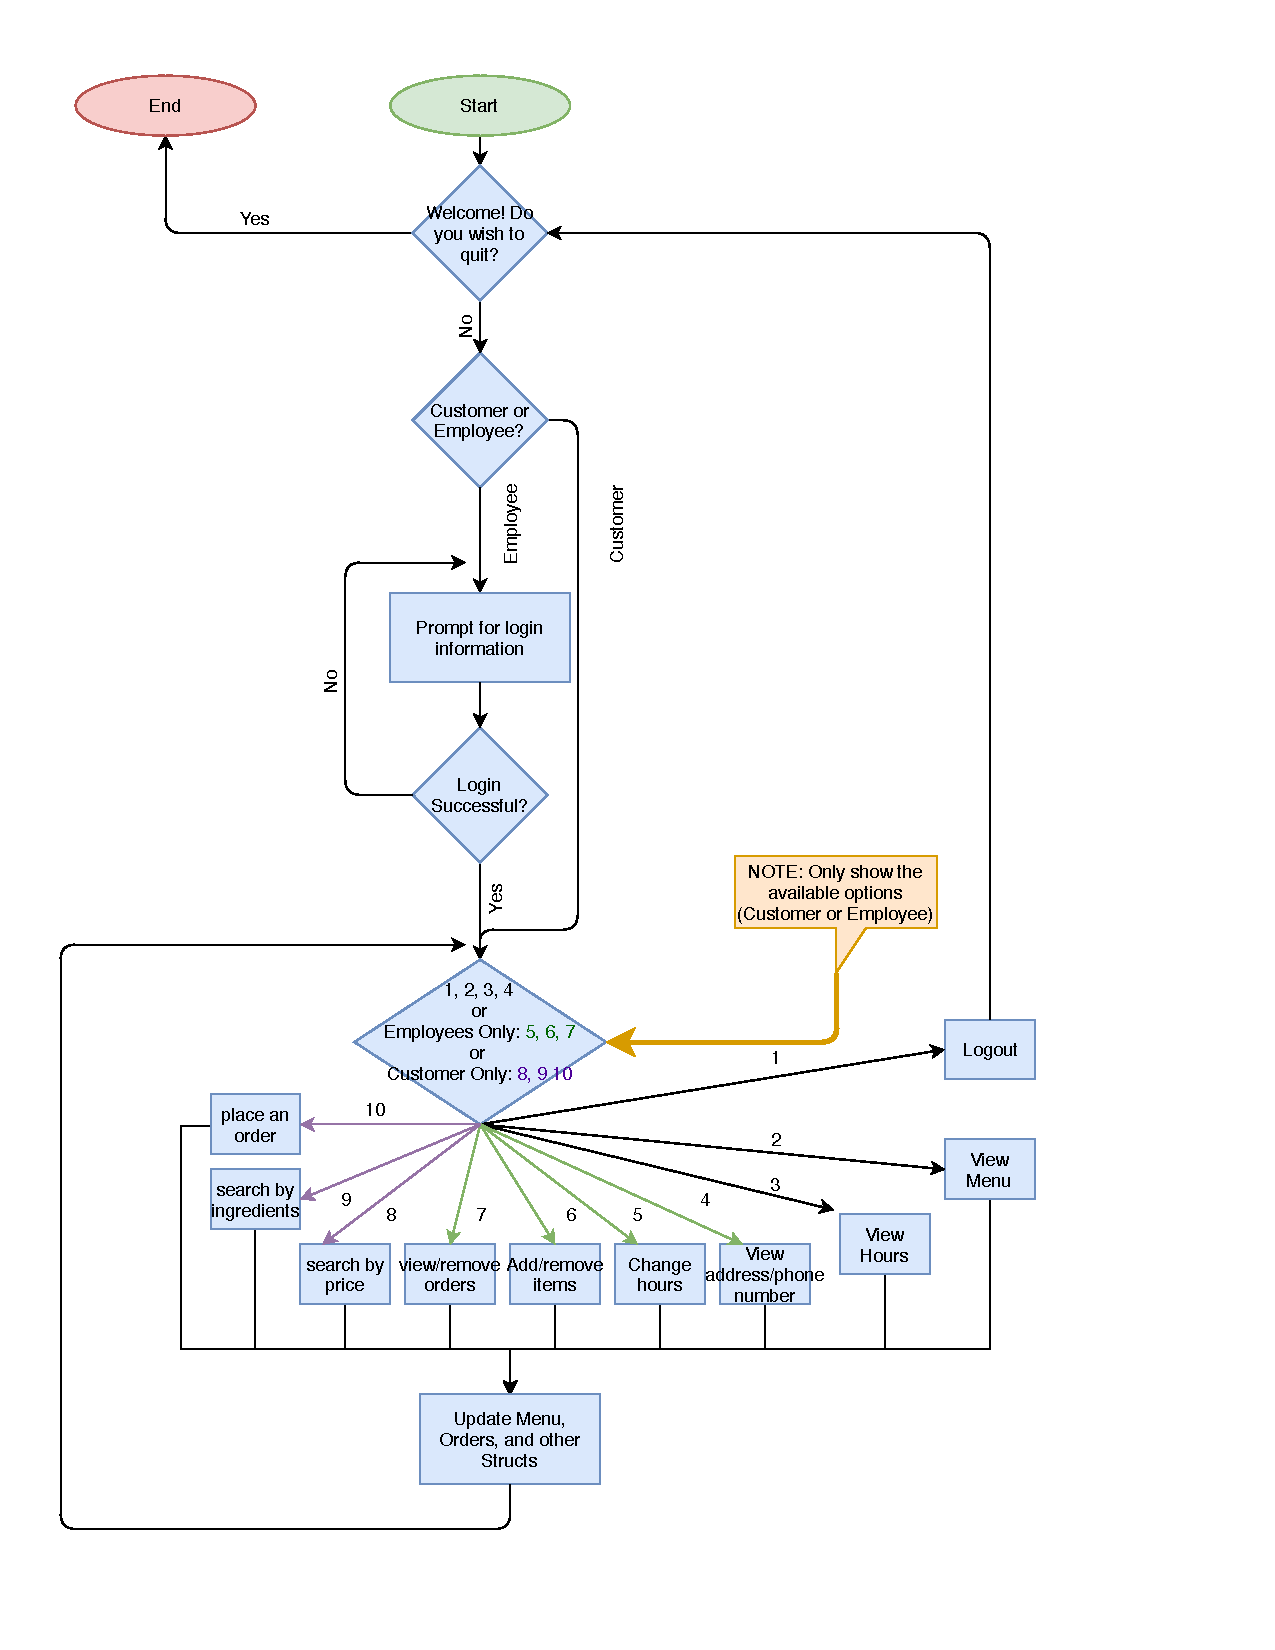
\includepdf{images/flow_chart.pdf}


\section*{Looking back / testing}

\textit{This includes any checking/self-reflection you did while solving the
  problem, which includes using a calculator to make sure the output is correct,
  testing to make sure your code executes correctly and behaves the way you
  expect under specific circumstances, using sources of information to make
  sense of the results, etc. However, you need to think about the input prior to
  implementation!!!}\\
\vspace{5em}

\begin{center}
 \begin{tabular}{l|c|r} % <-- Alignments: 1st column left, 2nd middle and 3rd right, with vertical lines in between
   \textbf{Value} & \textbf{Expected} & \textbf{Met expectation?}\\
    &  &  \\
   \hline
   Incorrect id & could not find wizard. please try again  & \\
   Incorrect pass & Incorrect password Please try again & \\
   Incorrect pass (x3) & You failed to log in. (Quit program)  & \\
   Correct user and pass  &Login successful. Display wizard info & \\
   Test each sort option & Correctly sorts & \\
   Print to screen & correctly displays information & \\
   Print to file & correctly writes to file & \\
 \end{tabular}
\end{center} 






\end{document}





































